\begin{frame}
	\frametitle{Procedimento 03}
	\framesubtitle{Descrição}
	\only<1>{
		\begin{itemize}
			\item 300 testes aleatórios em cada caso.
			\item EER = equilibrio entre as taxas de falsos positivos e de falsos negativos.
			\item Em alguns casos o cálculo do EER necessitou mais iterações.
			\item 10\%, 20\%, 30\%, 40\% e 50\% da base de sinais reservados para treinamento.
		\end{itemize}
	}	
\end{frame}

\begin{frame}
	\frametitle{Procedimento 03}
	\framesubtitle{Tabela de resultados}
	\begin{table}[H]
	\newcommand{\mc}[3]{\multicolumn{#1}{#2}{#3}}
	\definecolor{tcA}{rgb}{0.65098,0.65098,0.65098}
	\definecolor{tcB}{rgb}{0.447059,0.74902,0.266667}
	\begin{center}
		\caption{Resultados da abordagem com SVM}
		\begin{tabular}{|p{0.15\linewidth}|p{0.11\linewidth}|p{0.11\linewidth}|p{0.11\linewidth}|p{0.14\linewidth}|p{0.14\linewidth}|}\hline
			% use packages: color,colortbl
			\rowcolor{tcA}
			\centering\textbf{$M$} & \centering\textbf{Acurácia mínima} & \centering\textbf{Acurácia máxima} & \centering\textbf{Média das acurácias} & \centering\textbf{Desvio padrão da acurácia} & \begin{center}\textbf{EER}\end{center}\\\hline
			
			\rowcolor{tcB}
			% Loads data from tables/results/paraconsistentPlane/distParacomFrom10.csv
			\csvreader[
			late after line=\\\hline\rowcolor{tcB},%
			separator=comma,
			]{tables/results/experiment02ResultsSVM.csv}{1=\eme,2=\minAccu,3=\maxAccu,4=\meanAccu,5=\stdDev,6=\eer}{\centering\eme\% & \centering\StrSubstitute[0]{\minAccu}{.}{,} & \centering\StrSubstitute[0]{\maxAccu}{.}{,} & \centering\StrSubstitute[0]{\meanAccu}{.}{,} & \centering\StrSubstitute[0]{\stdDev}{.}{,} & \StrSubstitute[0]{\eer}{.}{,}}
			
		\end{tabular}
		\label{tab:experiment03Results}
		\\Fonte: Elaborado pelo autor, 2021.
	\end{center}
\end{table}
\end{frame}

\begin{frame}
	\frametitle{Procedimento 03}
	\framesubtitle{Acurácias e EER para SVM}
	\only<1>{
		\begin{columns}
			\column{0.5\textwidth}
			\begin{figure}
				\centering
				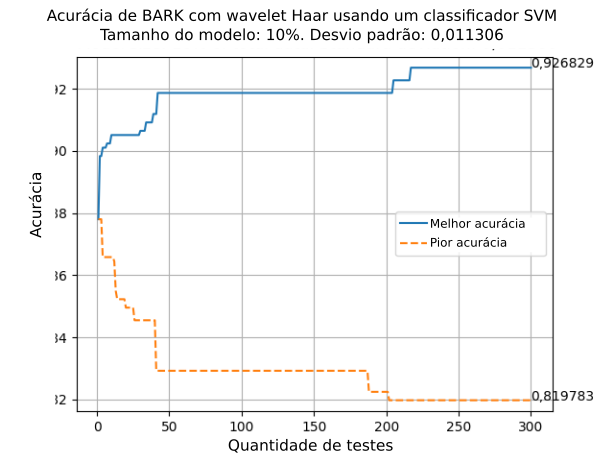
\includegraphics[width=\linewidth]{../monography/images/results/confusionMatrices/classifier_SVM_10}
				\caption{Acurácia \textit{X} quantidade de testes - SVM, modelo a 10\%}
			\end{figure}
			
			\column{0.5\textwidth}
			\begin{figure}
				\centering
				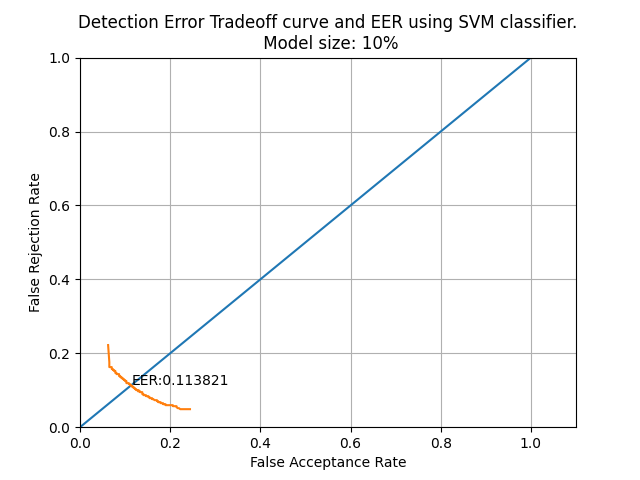
\includegraphics[width=\linewidth]{../monography/images/results/det/DET_SVM_10}
				\caption{Curva DET dos resultados de SVM, modelo a 10\%}
			\end{figure}
		\end{columns}
	}
	\only<2>{
		\begin{columns}
			\column{0.5\textwidth}
			\begin{figure}
				\centering
				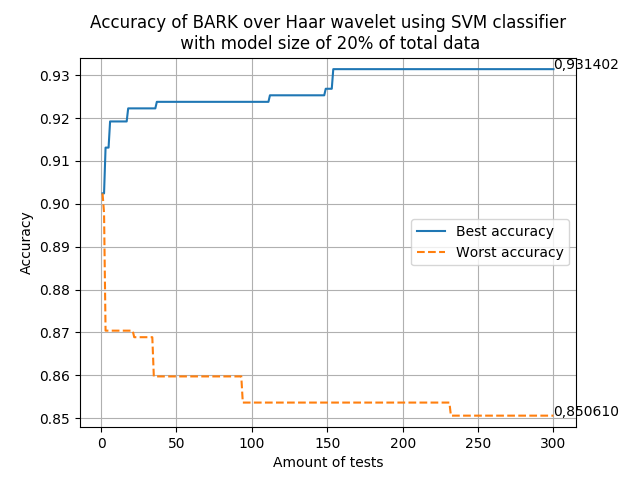
\includegraphics[width=\linewidth]{../monography/images/results/confusionMatrices/classifier_SVM_20}
				\caption{Acurácia \textit{X} quantidade de testes - SVM, modelo a 20\%}
			\end{figure}
			
			\column{0.5\textwidth}
			\begin{figure}
				\centering
				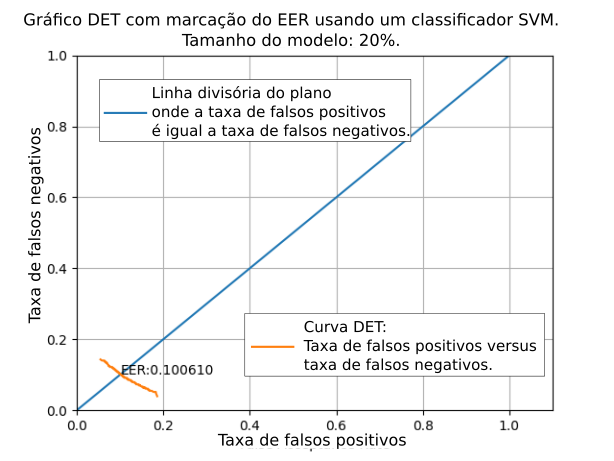
\includegraphics[width=\linewidth]{../monography/images/results/det/DET_SVM_20}
				\caption{Curva DET dos resultados de SVM, modelo a 20\%}
			\end{figure}
		\end{columns}
	}
	\only<3>{
		\begin{columns}
			\column{0.5\textwidth}
			\begin{figure}
				\centering
				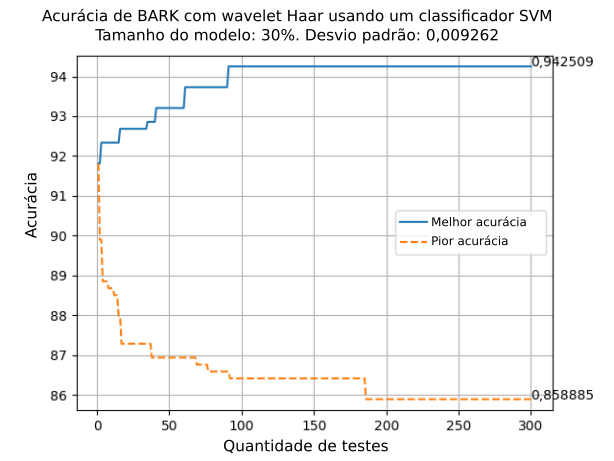
\includegraphics[width=\linewidth]{../monography/images/results/confusionMatrices/classifier_SVM_30}
				\caption{Acurácia \textit{X} quantidade de testes - SVM, modelo a 30\%}
			\end{figure}
			
			\column{0.5\textwidth}
			\begin{figure}
				\centering
				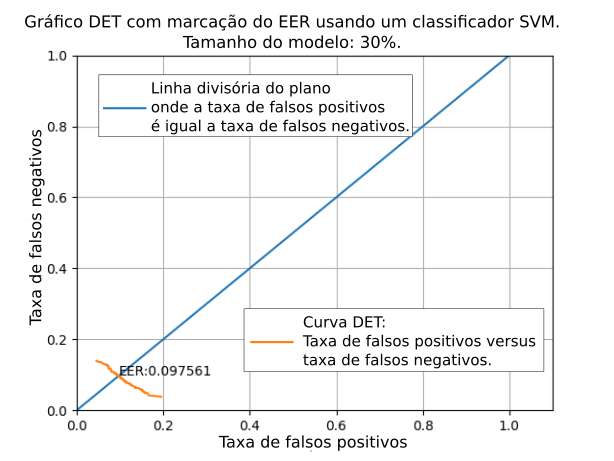
\includegraphics[width=\linewidth]{../monography/images/results/det/DET_SVM_30}
				\caption{Curva DET dos resultados de SVM, modelo a 30\%}
			\end{figure}
		\end{columns}
	}
	\only<4>{
		\begin{columns}
			\column{0.5\textwidth}
			\begin{figure}
				\centering
				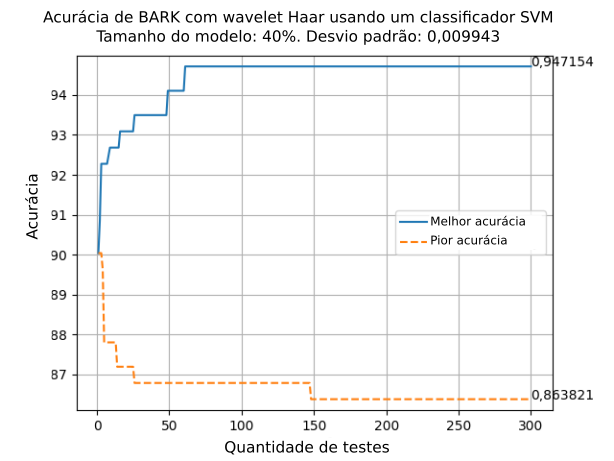
\includegraphics[width=\linewidth]{../monography/images/results/confusionMatrices/classifier_SVM_40}
				\caption{Acurácia \textit{X} quantidade de testes - SVM, modelo a 40\%}
			\end{figure}
			
			\column{0.5\textwidth}
			\begin{figure}
				\centering
				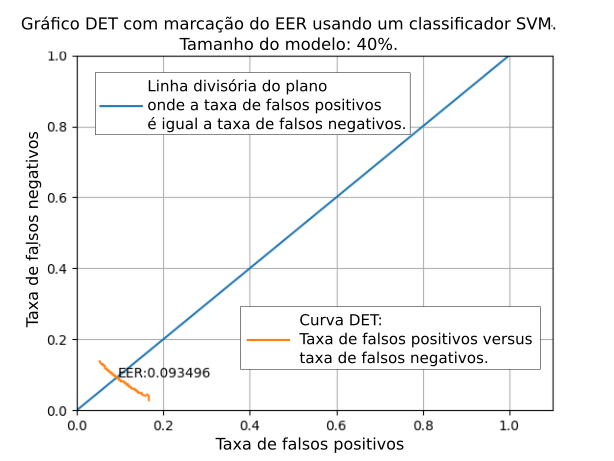
\includegraphics[width=\linewidth]{../monography/images/results/det/DET_SVM_40}
				\caption{Curva DET dos resultados de SVM, modelo a 40\%}
			\end{figure}
		\end{columns}
	}
	\only<5>{
		\begin{columns}
			\column{0.5\textwidth}
			\begin{figure}
				\centering
				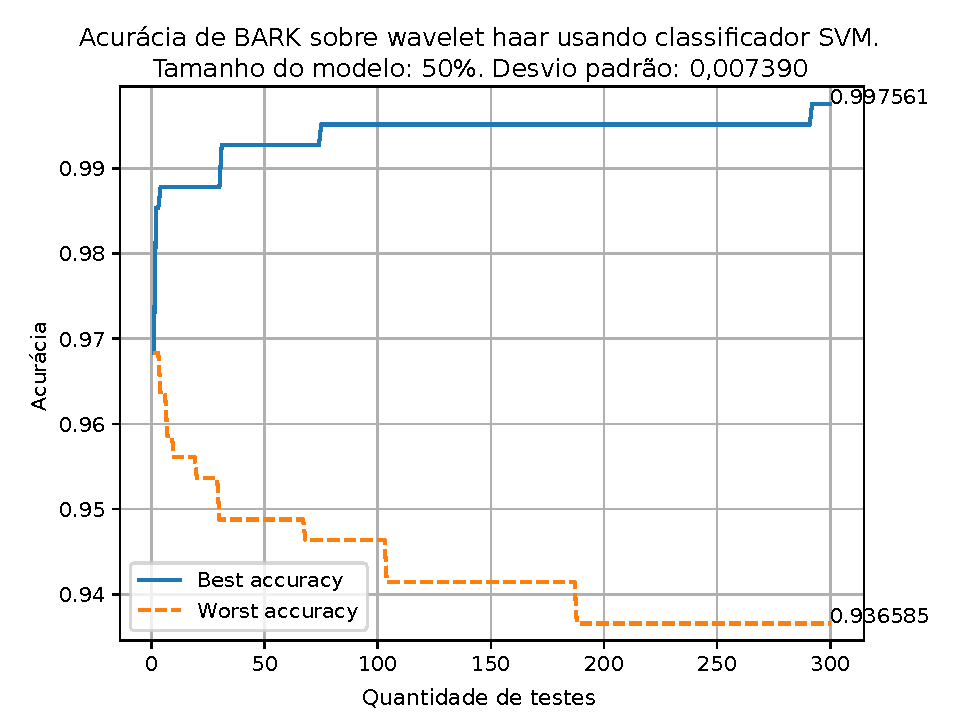
\includegraphics[width=\linewidth]{../monography/images/results/confusionMatrices/classifier_SVM_50}
				\caption{Acurácia \textit{X} quantidade de testes - SVM, modelo a 50\%}
			\end{figure}
			
			\column{0.5\textwidth}
			\begin{figure}
				\centering
				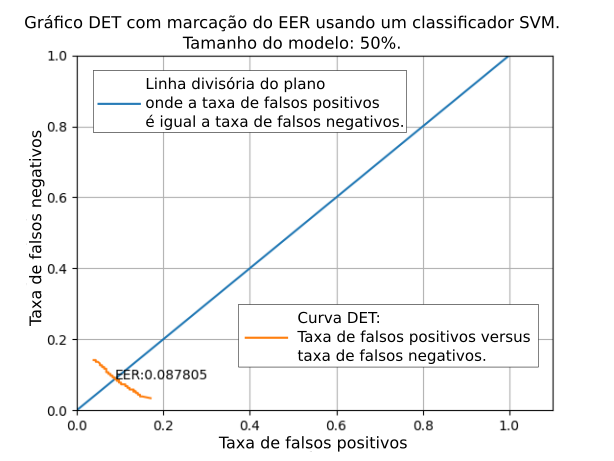
\includegraphics[width=\linewidth]{../monography/images/results/det/DET_SVM_50}
				\caption{Curva DET dos resultados de SVM, modelo a 50\%}
			\end{figure}
		\end{columns}
	}
\end{frame}

\begin{frame}
	\frametitle{Procedimento 03}
	\framesubtitle{Síntese}
	\par Dentre os testes realizados o melhores resultados foram:
	\begin{itemize}
		\item Acurácia: 0,953659.
		\item ERR: 0,087805.
	\end{itemize}
\end{frame}